%%%%%%%%%%%%%%%%%%%%%%%%%%%%%%%%%%%%%%%%%
% Beamer Presentation
% LaTeX Template
% Version 1.0 (10/11/12)
%
% This template has been downloaded from:
% http://www.LaTeXTemplates.com
%
% License:
% CC BY-NC-SA 3.0 (http://creativecommons.org/licenses/by-nc-sa/3.0/)
%
%%%%%%%%%%%%%%%%%%%%%%%%%%%%%%%%%%%%%%%%%

%----------------------------------------------------------------------------------------
%	PACKAGES AND THEMES
%----------------------------------------------------------------------------------------

\documentclass{beamer}

\mode<presentation> {

% The Beamer class comes with a number of default slide themes
% which change the colors and layouts of slides. Below this is a list
% of all the themes, uncomment each in turn to see what they look like.

%\usetheme{default}
%\usetheme{AnnArbor}
%\usetheme{Antibes}
%\usetheme{Bergen}
%\usetheme{Berkeley}
%\usetheme{Berlin}
%\usetheme{Boadilla}
%\usetheme{CambridgeUS}
%\usetheme{Copenhagen}
%\usetheme{Darmstadt}
%\usetheme{Dresden}
%\usetheme{Frankfurt}
%\usetheme{Goettingen}
%\usetheme{Hannover}
%\usetheme{Ilmenau}
%\usetheme{JuanLesPins}
%\usetheme{Luebeck}
\usetheme{Madrid}
%\usetheme{Malmoe}
%\usetheme{Marburg}
%\usetheme{Montpellier}
%\usetheme{PaloAlto}
%\usetheme{Pittsburgh}
%\usetheme{Rochester}
%\usetheme{Singapore}
%\usetheme{Szeged}
%\usetheme{Warsaw}

% As well as themes, the Beamer class has a number of color themes
% for any slide theme. Uncomment each of these in turn to see how it
% changes the colors of your current slide theme.

%\usecolortheme{albatross}
%\usecolortheme{beaver}
%\usecolortheme{beetle}
%\usecolortheme{crane}
%\usecolortheme{dolphin}
%\usecolortheme{dove}
%\usecolortheme{fly}
%\usecolortheme{lily}
%\usecolortheme{orchid}
%\usecolortheme{rose}
%\usecolortheme{seagull}
%\usecolortheme{seahorse}
%\usecolortheme{whale}
%\usecolortheme{wolverine}

%\setbeamertemplate{footline} % To remove the footer line in all slides uncomment this line
%\setbeamertemplate{footline}[page number] % To replace the footer line in all slides with a simple slide count uncomment this line

%\setbeamertemplate{navigation symbols}{} % To remove the navigation symbols from the bottom of all slides uncomment this line
}

\usepackage{graphicx} % Allows including images
\usepackage{booktabs} % Allows the use of \toprule, \midrule and \bottomrule in tables
\usepackage{subfigure} % Allows to use subfigure in images
\usepackage{xcolor} % Allows to use text color
\usepackage{galois} % Allows little circle
\usepackage{amsmath,amsthm,amsfonts,amssymb,amscd}
\usepackage{multicol} %Allows multi columns in content page.
\usepackage{amssymb} %Allows empty set
\usepackage[linesnumbered,ruled]{algorithm2e} %Allows pseudocode

\usepackage{tikz}
\usetikzlibrary{shapes.geometric}
\usetikzlibrary{arrows,positioning, calc}
\tikzstyle{vertex}=[draw,fill=black!15,circle,minimum size=12pt,inner sep=0pt]
\tikzstyle{itria}=[draw,dashed,shape border uses incircle,
  isosceles triangle,shape border rotate=90,yshift=-1.45cm]

%----------------------------------------------------------------------------------------
%	TITLE PAGE
%----------------------------------------------------------------------------------------

\title[Trees Edit Distance]{Optimal Decomposition Strategy For Tree Edit Distance} % The short title appears at the bottom of every slide, the full title is only on the title page

\author{Shaofeng Jiang} % Your name
\institute[Western University] % Your institution as it will appear on the bottom of every slide, may be shorthand to save space
{
Supervised By Dr. Kaizhong Zhang\\ % Your institution for the title page
\medskip
\textit{sjian7@uwo.ca} % Your email address
}
\date{\today} % Date, can be changed to a custom date

\begin{document}

\begin{frame}
\titlepage % Print the title page as the first slide
\end{frame}

\begin{frame}
\frametitle{Overview} % Table of contents slide, comment this block out to remove it
%\begin{multicols}{2}
  \tableofcontents
%\end{multicols}
%\tableofcontents % Throughout your presentation, if you choose to use \section{} and \subsection{} commands, these will automatically be printed on this slide as an overview of your presentation
\end{frame}

%----------------------------------------------------------------------------------------
%	PRESENTATION SLIDES
%----------------------------------------------------------------------------------------

%------------------------------------------------
\section{Introduction}
\begin{frame}
\frametitle{Ordered Labelled Tree }
An ordered labelled tree is a tree in which the nodes are labeled and the left-to-right order among siblings is significant. 
\begin{figure}
	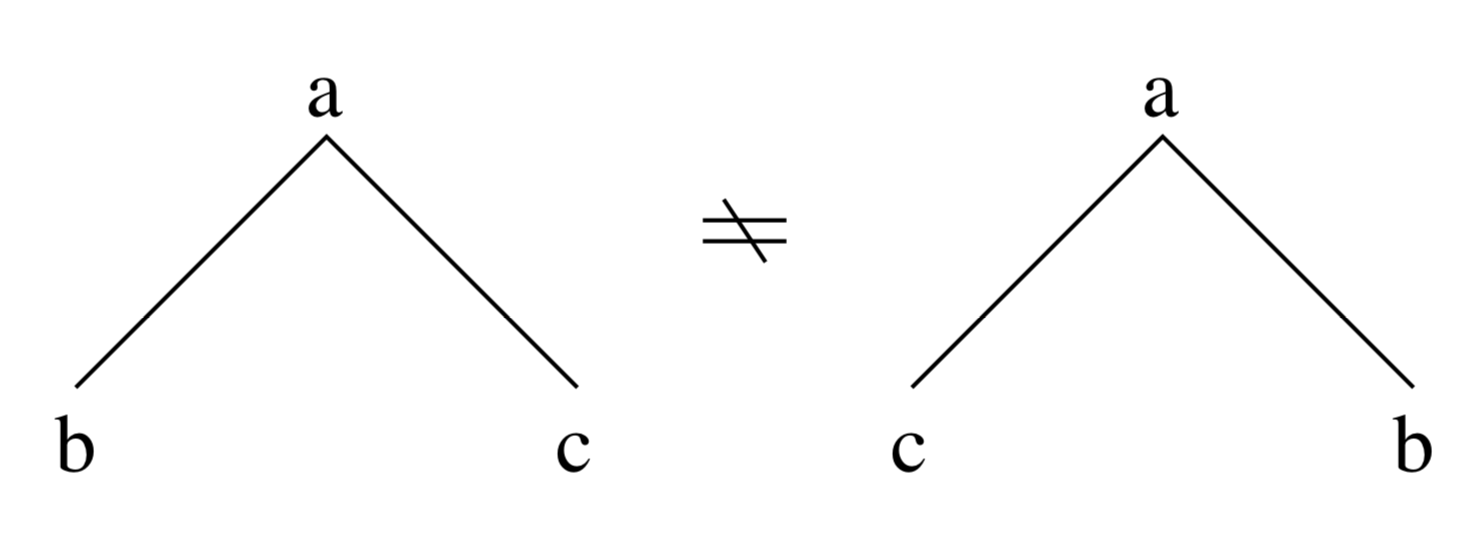
\includegraphics[width=0.6\linewidth]{OrderedLabelledTree}
	\label{Ordered Labelled Tree} 
	\caption{Ordered Labelled Tree}
	\centering
\end{figure}
The ordered labelled tree can represent:
\begin{itemize}
\item an XML document
\item a natural language parse 
\item RNA secondary structure
\item and so on...
\end{itemize}
\end{frame}
%------------------------------------------------
\begin{frame}
\frametitle{Tree Edit Distance}
\begin{itemize}
\item The string edit distance is the minimum cost to transform one string to another.
\begin{itemize}
\item Align two sequences of nucleotides
\begin{figure}
	
\includegraphics[width=0.8\linewidth]{Sequence}
\end{figure}
\item Resulting alignment
\begin{figure}
	
\includegraphics[width=0.8\linewidth]{SequenceAfterAlign}
\end{figure}
\end{itemize}
\item The tree edit distance is introduced by Tai as a generalization of the string edit distance. 
\item The edit distance between two trees  $P$  and $D$  is the minimum cost to change $P $ to $D$  via a sequence of basic edit operations.
\end{itemize}
\end{frame}
%------------------------------------------------
\begin{frame}
\frametitle{Edit Operations}
\begin{itemize}
\item Three valid edit operations supported:
\begin{itemize}
\item \textbf{Substitution.} replace a label of a node by another label. 
\begin{figure}
	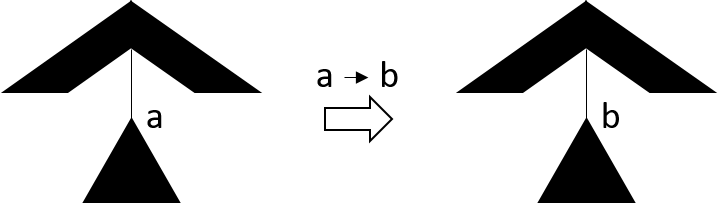
\includegraphics[width=0.4\linewidth]{Replacement}
	\label{Substitution} 
	\centering
\end{figure}
\item \textbf{Deletion.} deletion of a node
\begin{figure}
	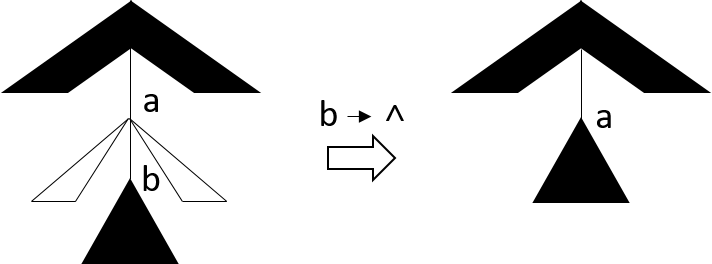
\includegraphics[width=0.4\linewidth]{Delete}
	\label{Deletion} 
	\centering
\end{figure}
\item \textbf{Insertion.} insertion of a node.
\begin{figure}
	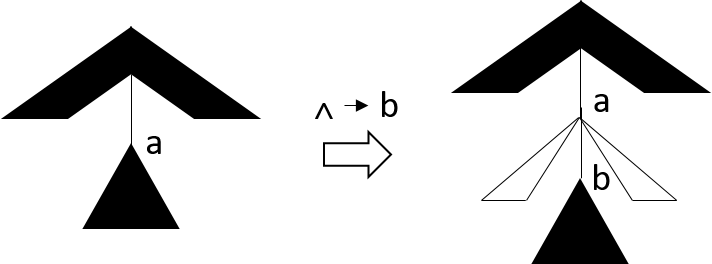
\includegraphics[width=0.4\linewidth]{Insertion}
	\label{Insertion} 
	\centering
\end{figure}
\end{itemize}
\end{itemize}
\end{frame}
%------------------------------------------------
\begin{frame}
\frametitle{Edit Operations}
\begin{figure}
	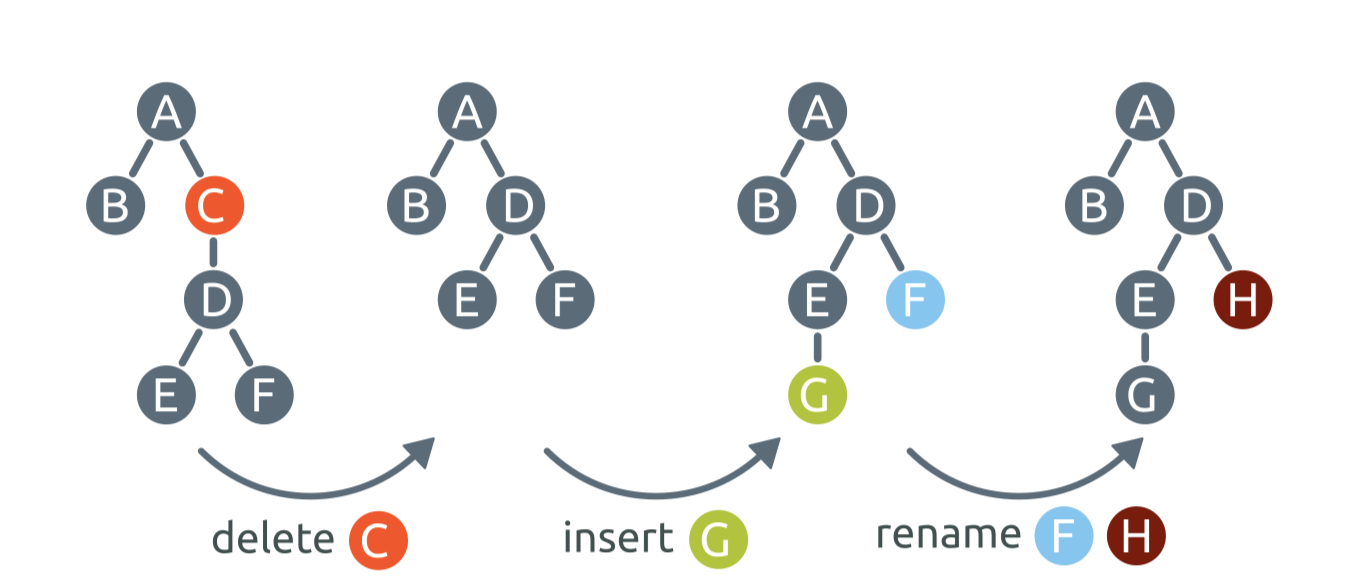
\includegraphics[width=1.0\linewidth]{EditExample}
	\label{Substitution} 
	\centering
\end{figure}
\end{frame}		
%------------------------------------------------
\begin{frame}
\frametitle{Cost of Edit Operations}
\begin{itemize}
\item Each edit operations has a cost. 
\item Let $\gamma$ be a cost function of each operations. The cost function $\gamma$ is a distance metric.
\begin{itemize}
\item $\gamma(a \to b)$ can be 1 or other user defined value.
\end{itemize}
\begin{figure}
	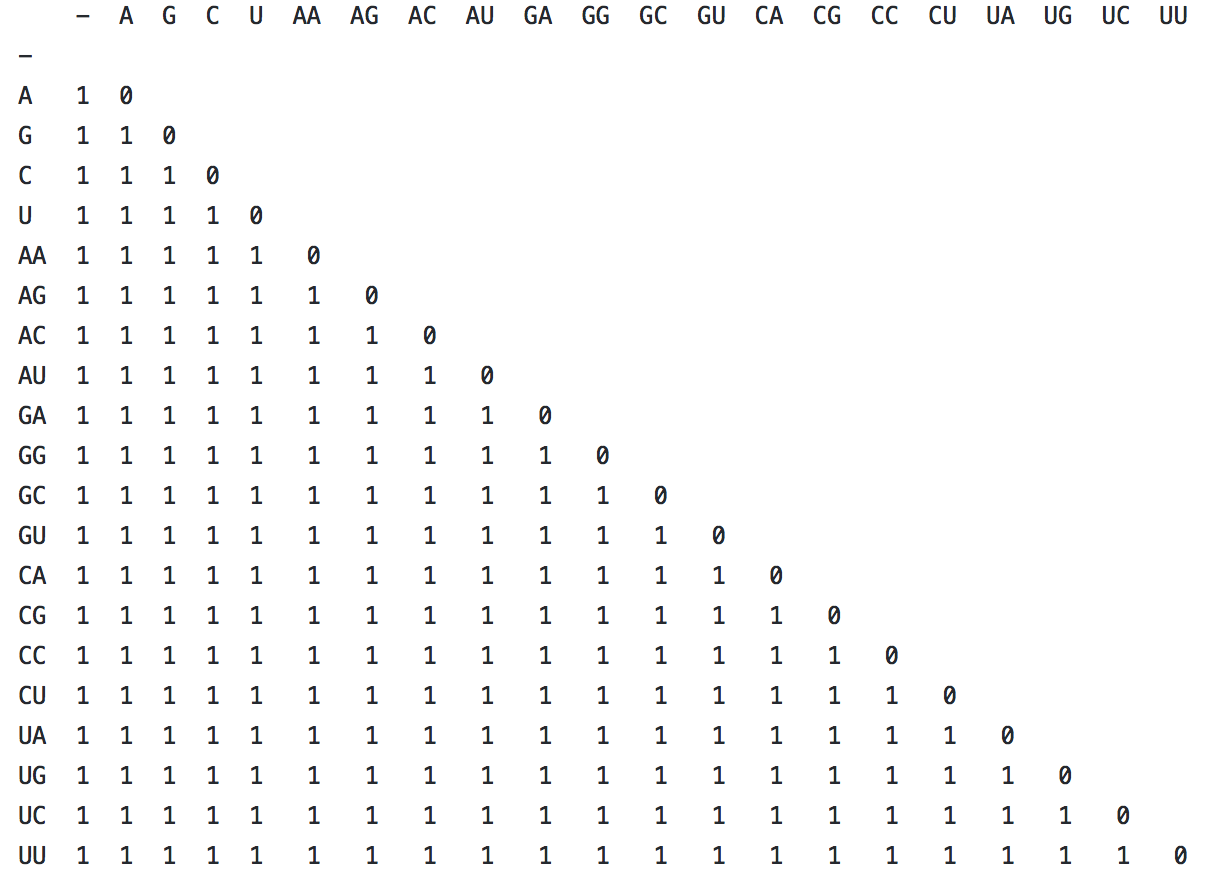
\includegraphics[width=0.6\linewidth]{distance}
	\label{Substitution} 
	\centering
\end{figure}
\item The edit distance is the sum of the cost of the minimum cost sequence.
\end{itemize}
\end{frame}
%------------------------------------------------
\begin{frame}
\frametitle{Mapping in Trees}
\begin{itemize}
\item Mapping between trees.% A sequence of edit operations can be used a mapping between trees to represent the alignment result.
\item The cost of a mapping is the sum of its insertion, deletion and substitutions.
\begin{figure}
	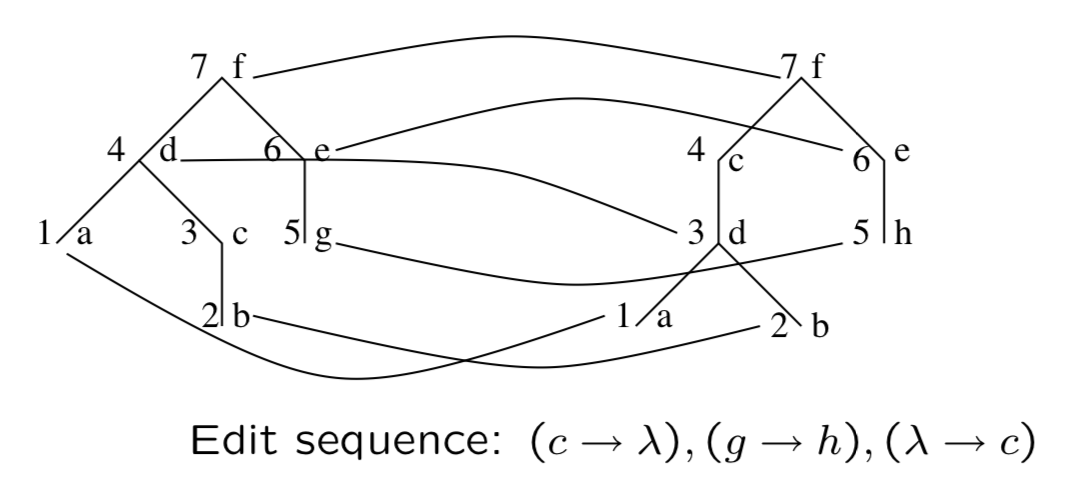
\includegraphics[width=0.7\linewidth]{EditDistance}
	\label{Edit Sequence} 
	\caption{The Edit Sequence and its Cost}
	\centering
\end{figure}
\end{itemize}
\end{frame}
%------------------------------------------------
\section{Notation}
\begin{frame}
\frametitle{Notation}
\begin{itemize}
\item \textbf{Tree} 
\begin{columns}[c] % The "c" option specifies centered vertical alignment while the "t" option is used for top vertical alignment
\column{.45\textwidth} % Left column and width
\begin{itemize}
\item $l(f)$
\begin{figure}
	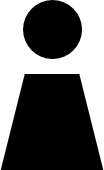
\includegraphics[width=0.2\linewidth]{Tree}
	\label{Tree} 
	\centering
\end{figure}
\end{itemize}
\column{.45\textwidth} % Left column and width
\begin{itemize}
\item $l(A_1 \comp A_2 \comp \cdots \comp A_n)$
\begin{figure}
	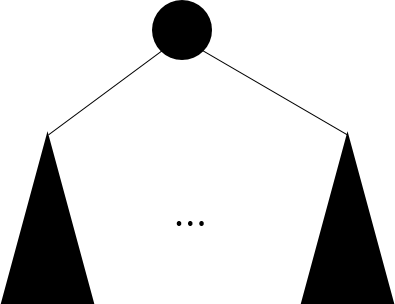
\includegraphics[width=0.5\linewidth]{Tree2}
	\label{Another Tree Representation} 
	\centering
\end{figure}
\end{itemize}
\end{columns}
\end{itemize}
Let T be a tree, 
\begin{columns}[c]
\column{.3\textwidth}
\begin{itemize}
\item \emph{$r(T)$}
\item \emph{$T^{\comp}$}
\item \emph{$lr(T)$}
\item \emph{$rr(T)$}
\end{itemize}
\column{.7\textwidth}
\begin{itemize}[]
\item[]  the root of T
\item[] $T - r(T)$
\item[]  the root of the leftmost tree in the forest $T^{\comp}$
\item[]  the root of the rightmost tree in the forest $T^{\comp}$
\end{itemize}
\end{columns}
\end{frame}
%------------------------------------------------
\begin{frame}
\frametitle{Notation}
\begin{itemize}
\item \textbf{Forest} 
\begin{columns}[c] % The "c" option specifies centered vertical alignment while the "t" option is used for top vertical alignment
\column{.45\textwidth} % Left column and width
\begin{itemize}
\item $l(f) \comp t$
\begin{figure}
	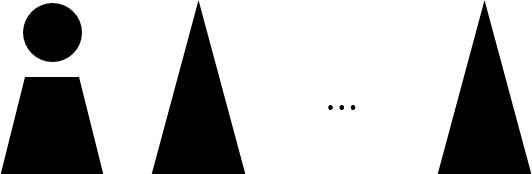
\includegraphics[width=0.8\linewidth]{Forest}
	\label{Forest} 
	\centering
\end{figure}
\end{itemize}
\column{.45\textwidth} % Left column and width
\begin{itemize}
\item $t \comp l(f)$
\begin{figure}
	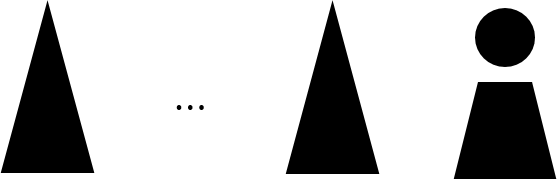
\includegraphics[width=0.8\linewidth]{Forest2}
	\label{Another Forest Representation} 
	\centering
\end{figure}
\end{itemize}
\end{columns}
\end{itemize}
Let F be a forest,
\begin{columns}[c]
\column{.3\textwidth}
\begin{itemize}
\item \emph{$\left\vert F \right\vert$}
\item \emph{$\#leaves(F)$}
\item \emph{$F(i)$}
\item \emph{$F - i$}
\item \emph{$lr(F)$}
\item \emph{$rr(F)$}
\end{itemize}
\column{.7\textwidth}
\begin{itemize}[]
\item[]  the number of nodes in the forest $F$
\item[]  the number of leaves in the forest $F$
\item[]  the sub-tree of F rooted at node i
\item[]  the forest after deleting node i
\item[]  the root of the leftmost tree in the forest $F$
\item[]  the root of the rightmost tree in the forest $F$
\end{itemize}
\end{columns}
\end{frame}
%------------------------------------------------
\section{Recursive Solution}
\begin{frame}
\frametitle{String Edit Distance and its Recursive Solution}
\begin{itemize}
\item String edit distance is the minimum cost to change one string to another via a sequence of basic edit operations.
\item The recursive solution of the string edit problem $d(S_1, S_2)$ is 
\begin{equation*}
d(S_1, S_2) = min \begin{cases}
	  	d(S_1 - u , S_2) + \delta(u, \varnothing) \\ 
      	d(S_1, S_2 - v) + \delta(\varnothing, v) \\ 
    	d(S_1 - u, S_2 - v) + \delta(u, v) & \\ 
    \end{cases}
\end{equation*}
\end{itemize}
\end{frame}
%------------------------------------------------
\begin{frame}
\frametitle{String Edit Distance and its Recursive Solution}
\begin{itemize}
\item If $u$ and $v$ is both the first element of string $S_1$ and $S_2$, then it is a leftmost decomposition.
\begin{figure}
	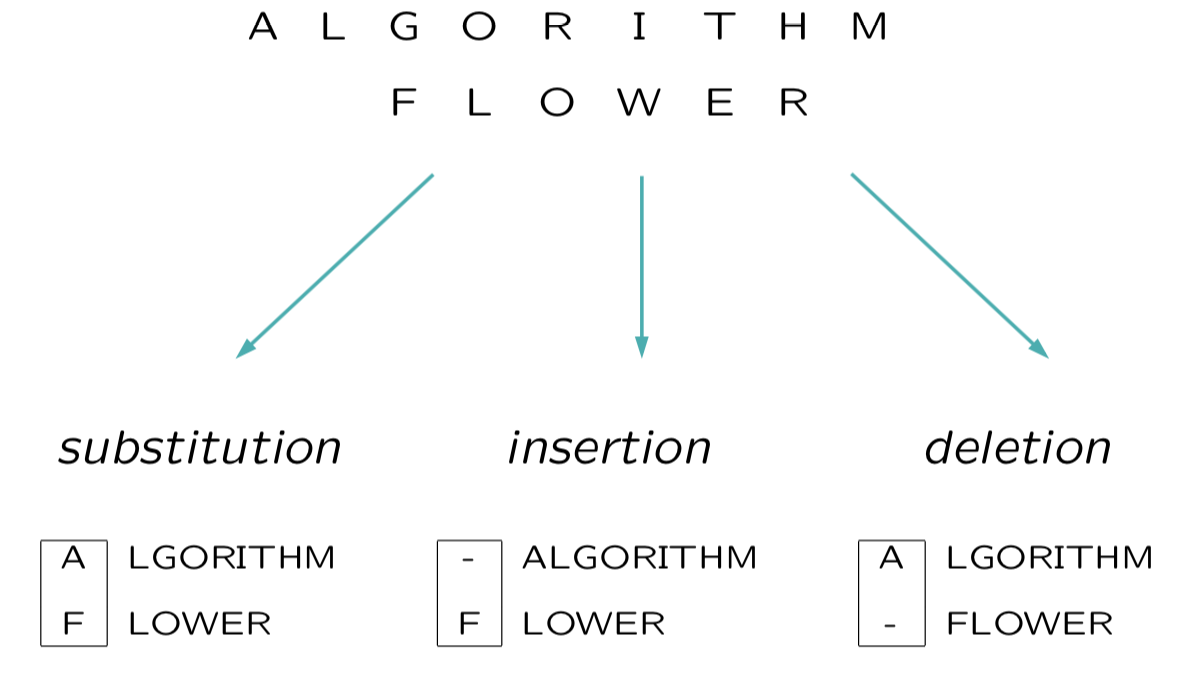
\includegraphics[width=0.4\linewidth]{StringRecursion1}
	\label{String Leftmost Decomposition} 
	\centering
\end{figure}
\item If $u$ and $v$ is both the last element of string $S_1$ and $S_2$, then it is a rightmost decomposition.
\begin{figure}
	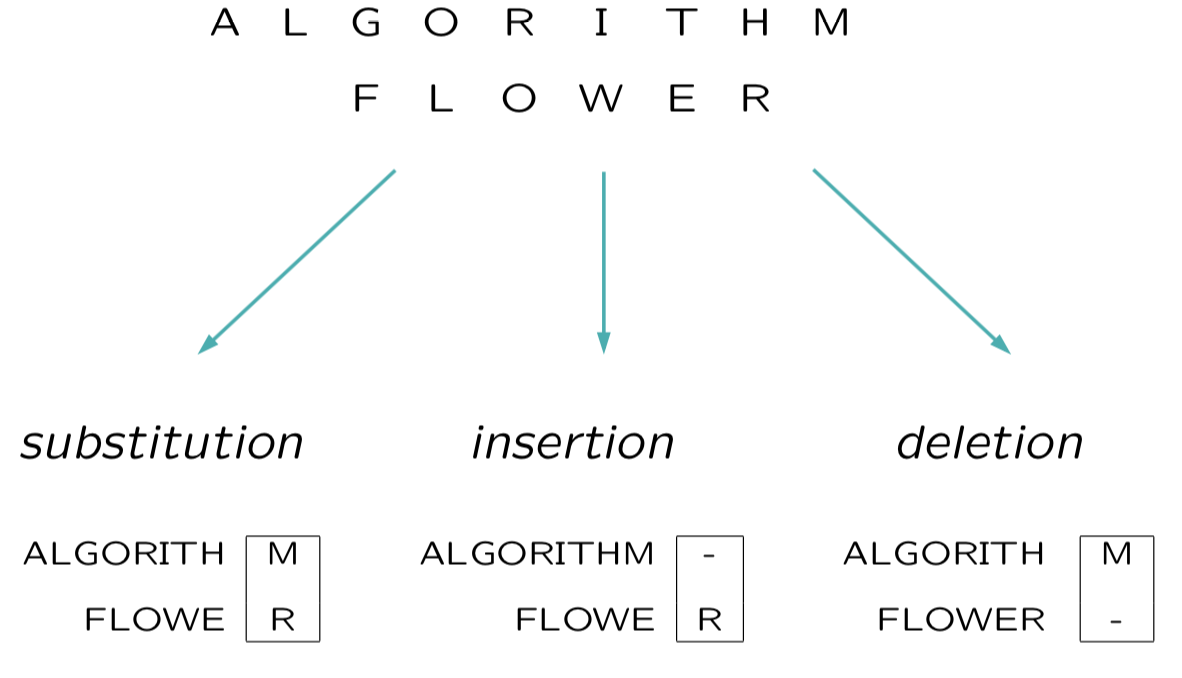
\includegraphics[width=0.4\linewidth]{StringRecursion2}
	\label{String Rightmost Decomposition} 
	\centering
\end{figure}
\end{itemize}
\end{frame}
%------------------------------------------------
\begin{frame}
\frametitle{Tree Edit Distance and its Recursive Solution}
For tree-to-tree distance,
Let $T_1$ and $T_2$ are both trees of the form $l(f)$ and $l'(f')$, 
\begin{align*}
d(l(f), l'(f')) = min \begin{cases}
	  	d(f, l'(f')) + \delta(l, \varnothing) \\ 
      	d(l(f), l'(f')) + \delta(\varnothing, l') \\ 
    	d(f, f') + \delta(l, l') & \\
    \end{cases}
\end{align*}
\begin{figure}
	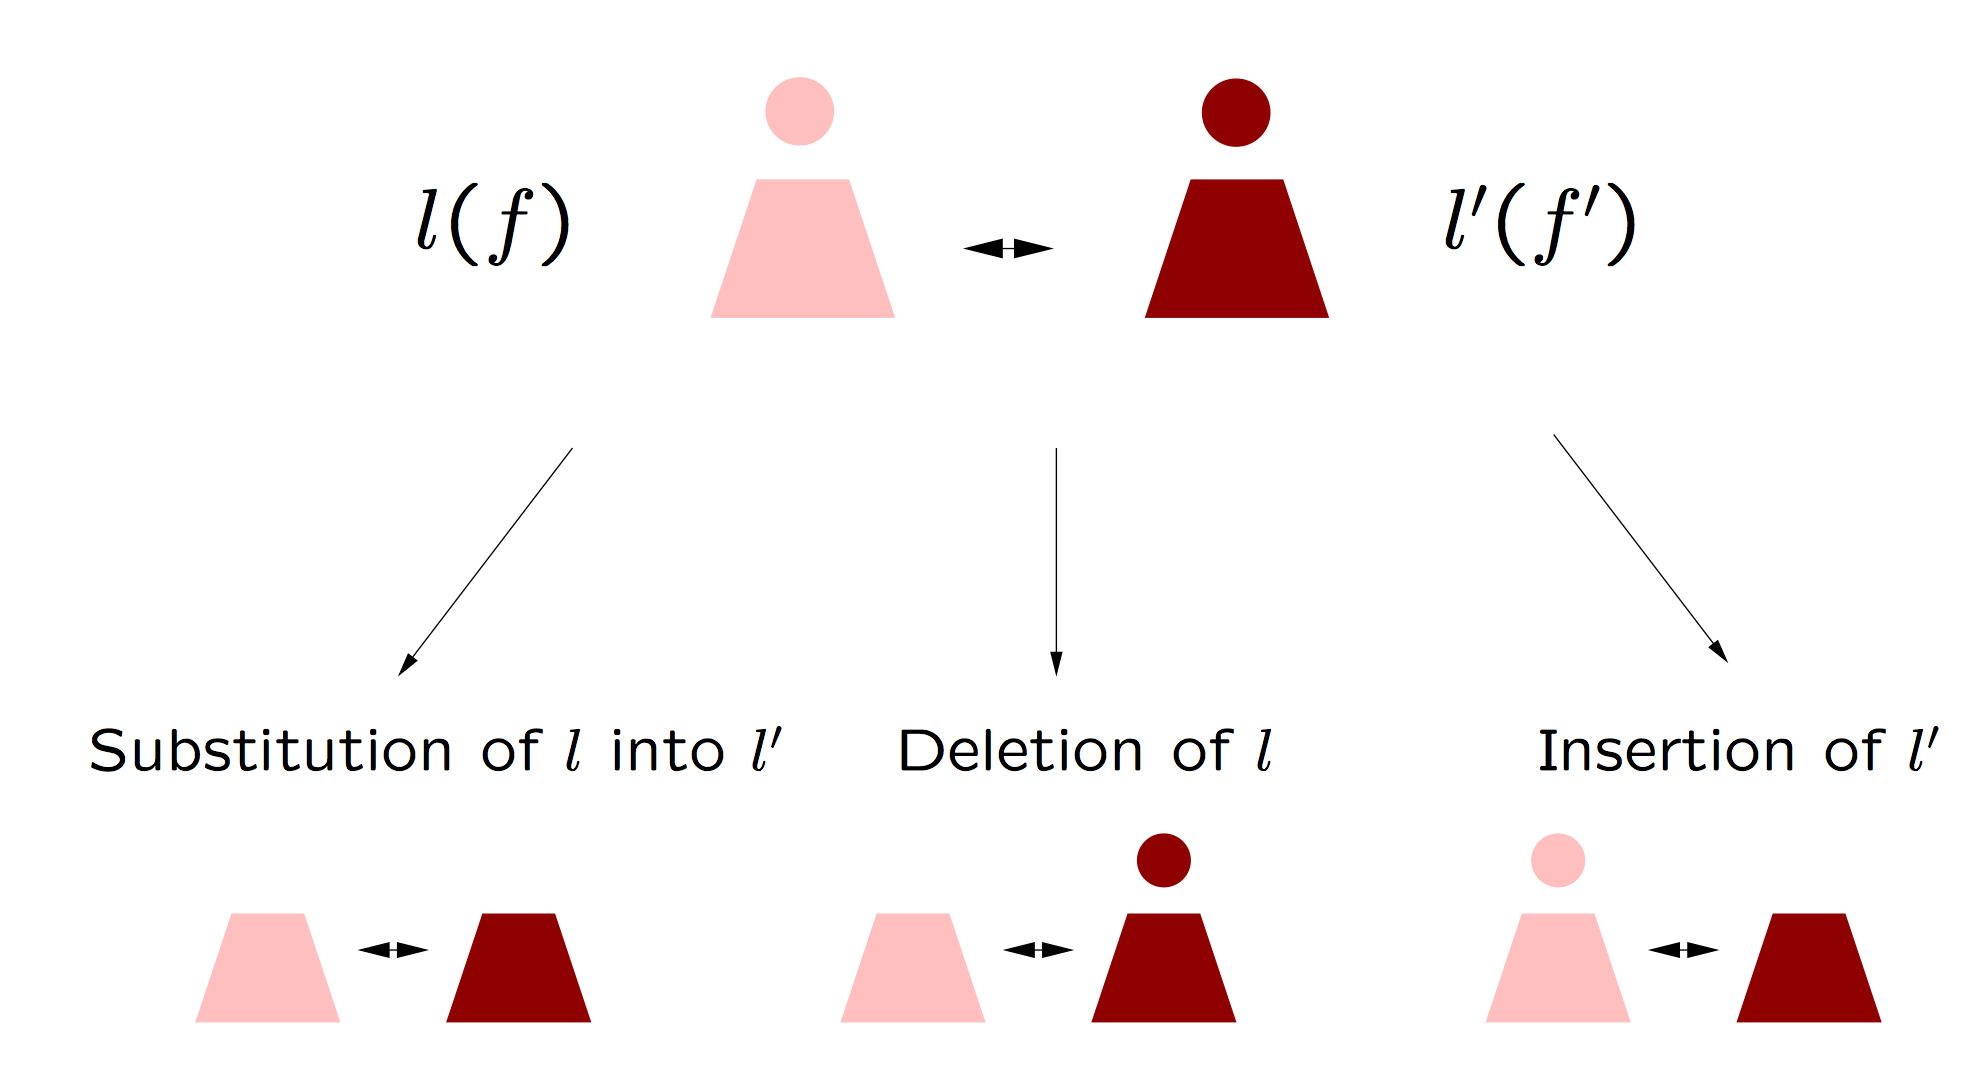
\includegraphics[width=0.6\linewidth]{TreeToTree}
	\label{Tree-to-Tree Edit Distance} 
	\caption{Tree-to-Tree Edit Distance}
	\centering
\end{figure}
\end{frame}
%------------------------------------------------
\begin{frame}
\frametitle{Tree Edit Distance and its Recursive Solution}
For forest-to-forest distance,
Let $F_1$ and $F_2$ are both trees of the form $l(f) \comp t$ and $l'(f') \comp t'$, 
\begin{align*}
d(l(f) \comp t, l'(f') \comp t') = min \begin{cases}
	  	d(f \comp t, l'(f') \comp t') + \delta(l, \varnothing) \\ 
      	d(l(f) \comp t, f' \comp t') + \delta(\varnothing, l') \\ 
    	d(t, t') + d(l(f), l'(f')) & \\
    \end{cases}
\end{align*}
\begin{figure}
	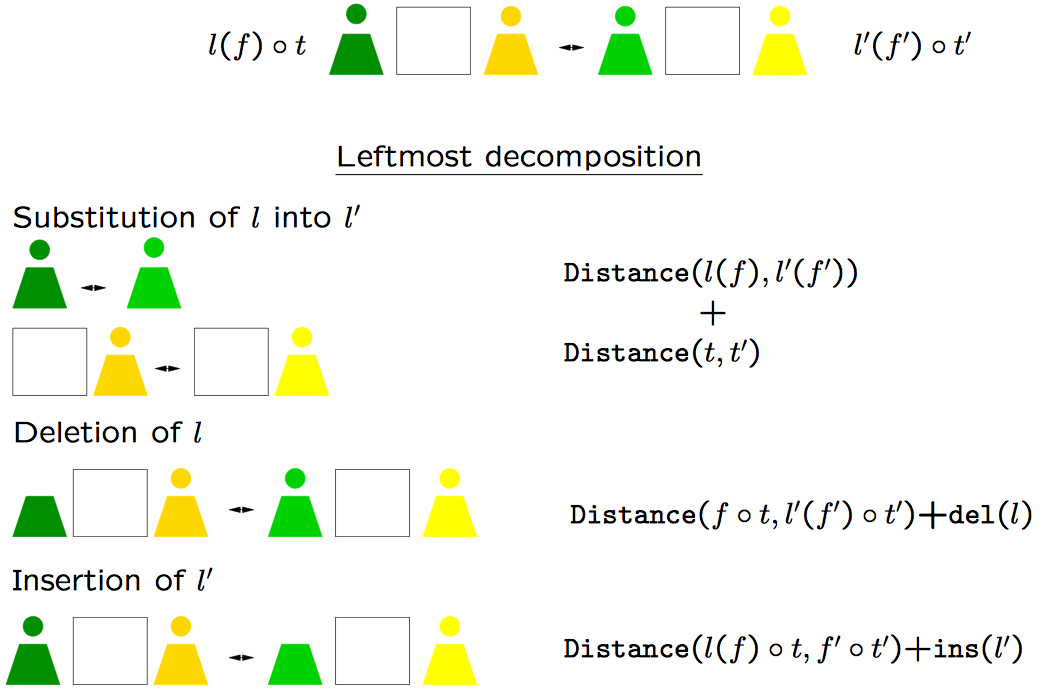
\includegraphics[width=0.6\linewidth]{ForestLeftmostDecomposition}
	\label{Forest-to-Forest Edit Distance} 
	\caption{Forest-to-Forest Edit Distance}
	\centering
\end{figure}
\end{frame}
%------------------------------------------------
\begin{frame}
\frametitle{Tree Edit Distance and its Recursive Solution}
For forest-to-forest distance,
Let $F_1$ and $F_2$ are both trees of the form $l(f) \comp t$ and $l'(f') \comp t'$, 
\begin{align*}
d(t \comp l(f), t' \comp l'(f')) = min \begin{cases}
	  	d(t  \comp f, t' \comp l'(f')) + \delta(l, \varnothing) \\ 
      	d(t \comp l(f), t'  \comp f') + \delta(\varnothing, l') \\ 
    	d(t, t') + d(l(f), l'(f')) & \\
    \end{cases}
\end{align*}
\begin{figure}
	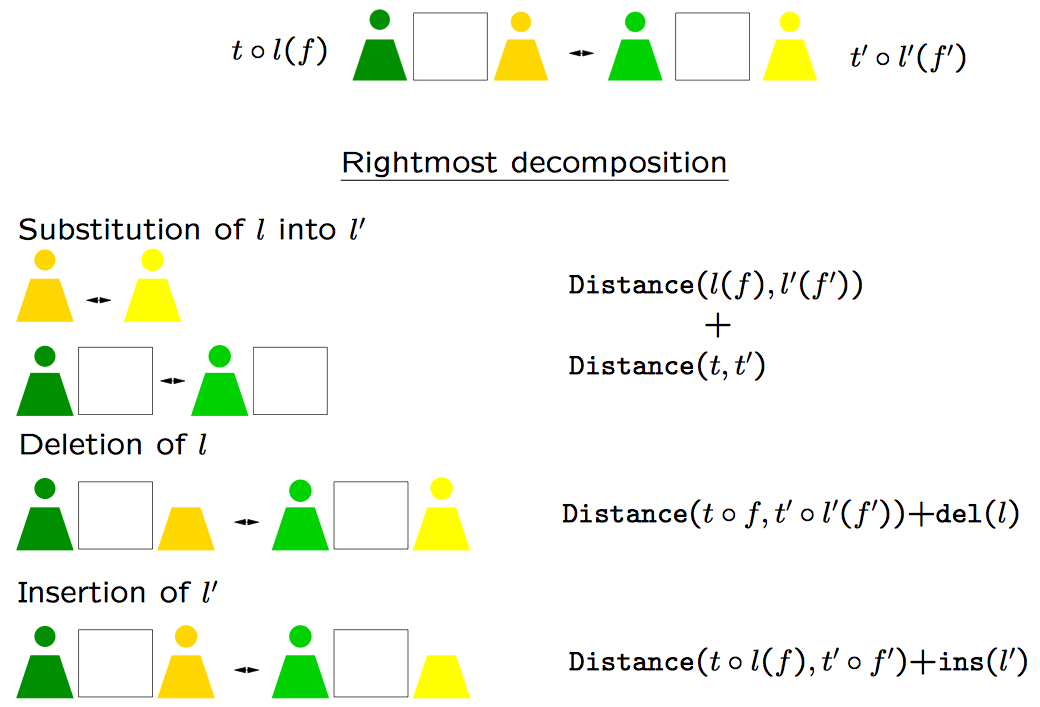
\includegraphics[width=0.55\linewidth]{ForestRightmostDecomposition}
	\label{Forest-to-Forest Edit Distance} 
	\caption{Forest-to-Forest Edit Distance}
	\centering
\end{figure}
\end{frame}
%------------------------------------------------
\begin{frame}
\frametitle{Relevant Sub-forests and Full Decomposition}
\begin{itemize}
\item  Relevant sub-forests
\begin{figure}
	%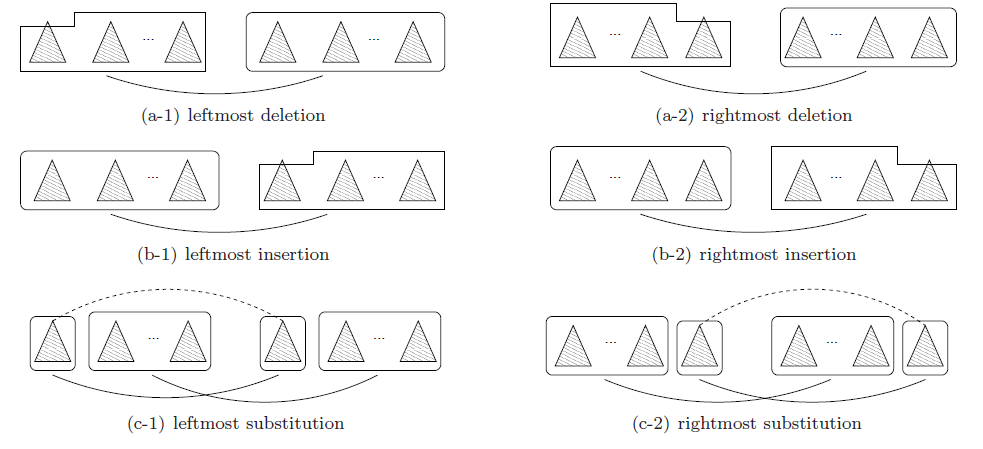
\includegraphics[width=0.7\linewidth]{LeftRightDecomposition}
	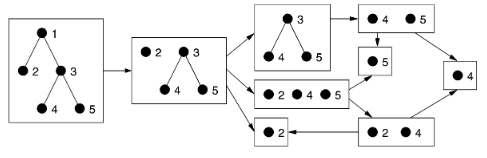
\includegraphics[width=0.6\linewidth]{LeftmostPathDecomposition}
	\centering
\end{figure}
\item Full decomposition
\begin{figure}
	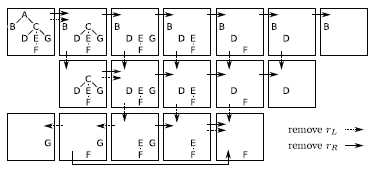
\includegraphics[width=0.6\linewidth]{FullDecomposition}
	\centering
\end{figure}
\end{itemize}
\end{frame}
%------------------------------------------------
\begin{frame}
\frametitle{Root-leaf Path and Relevant Sub-trees}
\begin{itemize}
\item Root-leaf path
\begin{figure}
	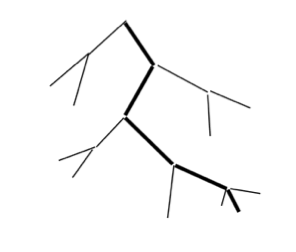
\includegraphics[width=0.2\linewidth]{RootLeafPath}
	\centering
\end{figure}
\item Relevant sub-trees
\begin{figure}
	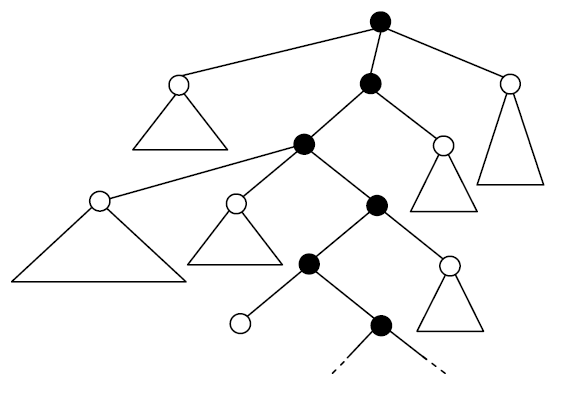
\includegraphics[width=0.3\linewidth]{RelevantSubtrees}
	\centering
\end{figure}
\item Path decomposition
\begin{figure}
	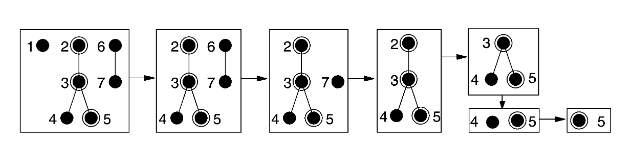
\includegraphics[width=0.6\linewidth]{KleinAlgorithmExample}
	\centering
\end{figure}
\end{itemize}
\end{frame}
%------------------------------------------------
\begin{frame}
\frametitle{Tree Indexing}
\begin{itemize}
\item $preOrder\_left\_to\_right\ \to\ preL\ $
\item $preOrder\_right\_to\_left\ \to\ preR\ $
\item $postOrder\_left\_to\_right\ \to\ postL\ $
\item $postOrder\_right\_to\_left\ \to\ postR\ $
\end{itemize}
Consider a tree T(preL, preR, postL, postR)

\begingroup

\centering
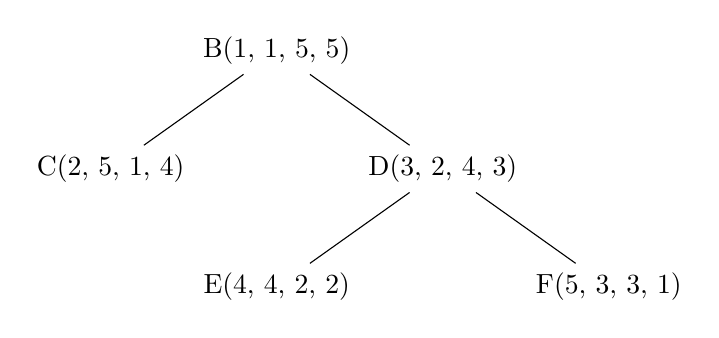
\begin{tikzpicture}[sibling distance=12em]
  \node {B(1, 1, 5, 5)}
    child {node {C(2, 5, 1, 4)}
    }
    child {node {D(3, 2, 4, 3)}
      child{node{E(4, 4, 2, 2)}}
      child {node {F(5, 3, 3, 1)}}
    };
\end{tikzpicture}

\endgroup
\textbf{Note:}
\begin{itemize}
\item $preL + postR= treeSize + 1$
\item $preR + postL= treeSize + 1$
\end{itemize}
\end{frame}
%------------------------------------------------
\begin{frame}
\frametitle{Bottom-up Enumeration}
Two orders of the enumeration of the full decomposition:
\begin{itemize}
\item Prefix-suffix order%enumerate the rightmost root in LR-postorder and fix it, then enumerate the leftmost root in LR-postorder.
\begin{figure}
	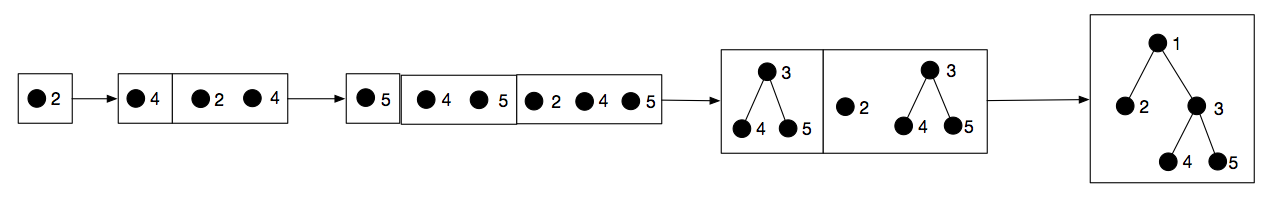
\includegraphics[width=1.0\linewidth]{PrefixSuffix}
	\centering
\end{figure}
\item Suffix-prefix order%enumerate the leftmost root in RL-postorder and fix it, then enuemrate the leftmost root in RL-postorder.
\begin{figure}
	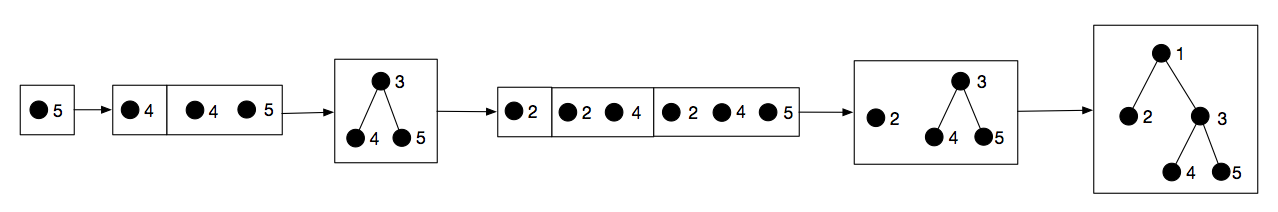
\includegraphics[width=1.0\linewidth]{SuffixPrefix}
	\centering
\end{figure}
\end{itemize}
\end{frame}
%------------------------------------------------
\section{Algorithms for the Tree Editing Distance}
\subsection{A Simple Algorithm}
\begin{frame}
\frametitle{A Simple Algorithm}
\textbf{Main Idea:}

Enumerate each pairs of sub-forests in tree A and B in prefix-suffix post order or suffix-prefix post order.

\textbf{Pseudocode:}
\begin{figure}
	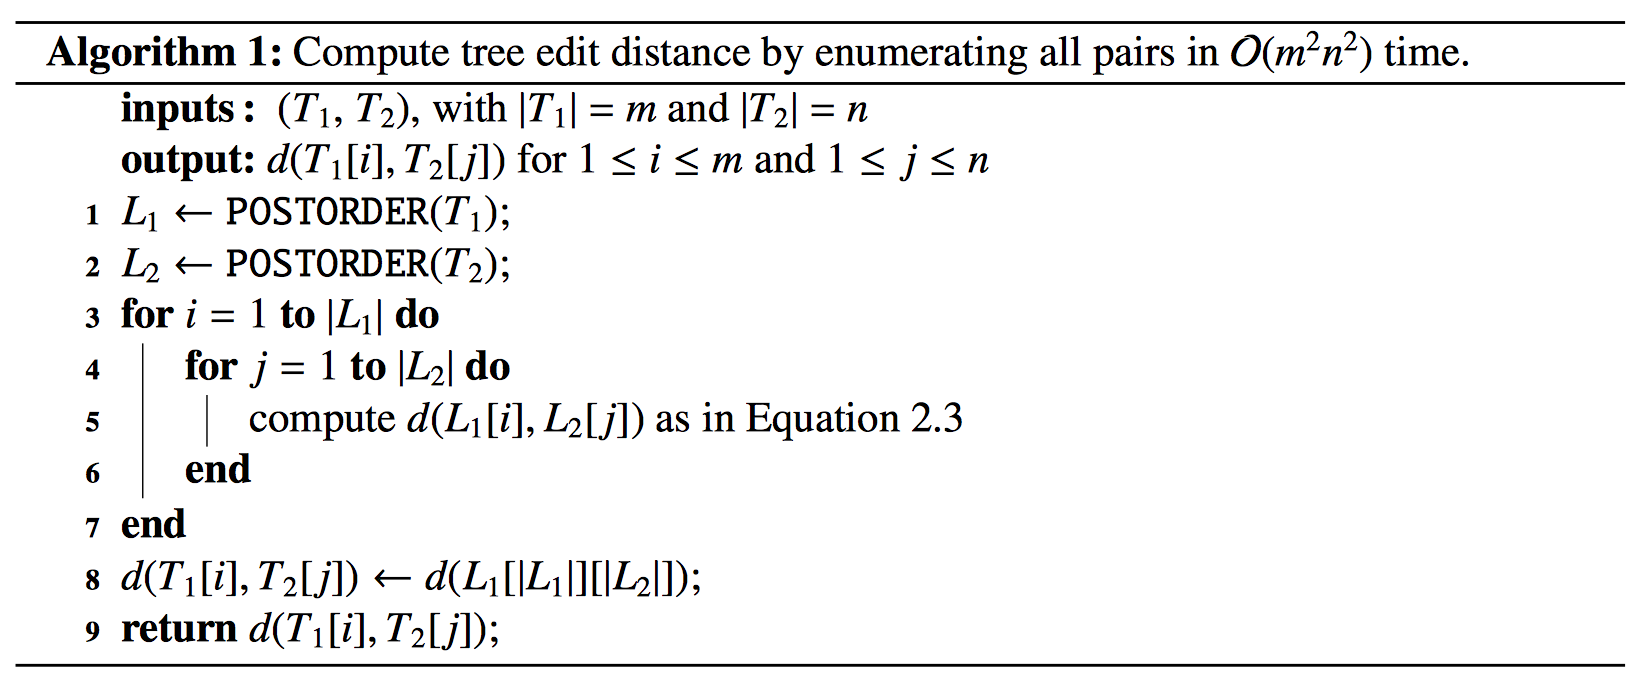
\includegraphics[width=1.0\linewidth]{SimpleAlgorithm}
	\centering
\end{figure}
\end{frame}

%------------------------------------------------
\begin{frame}
\frametitle{A Simple Algorithm}
\textbf{Implementation:}
\begin{itemize}
\item Implemented in dynamic programming.
\item Runs in $\mathcal{O}(m^2n^2)$ time using $\mathcal{O}(m^2n^2)$ space.
\begin{figure}
	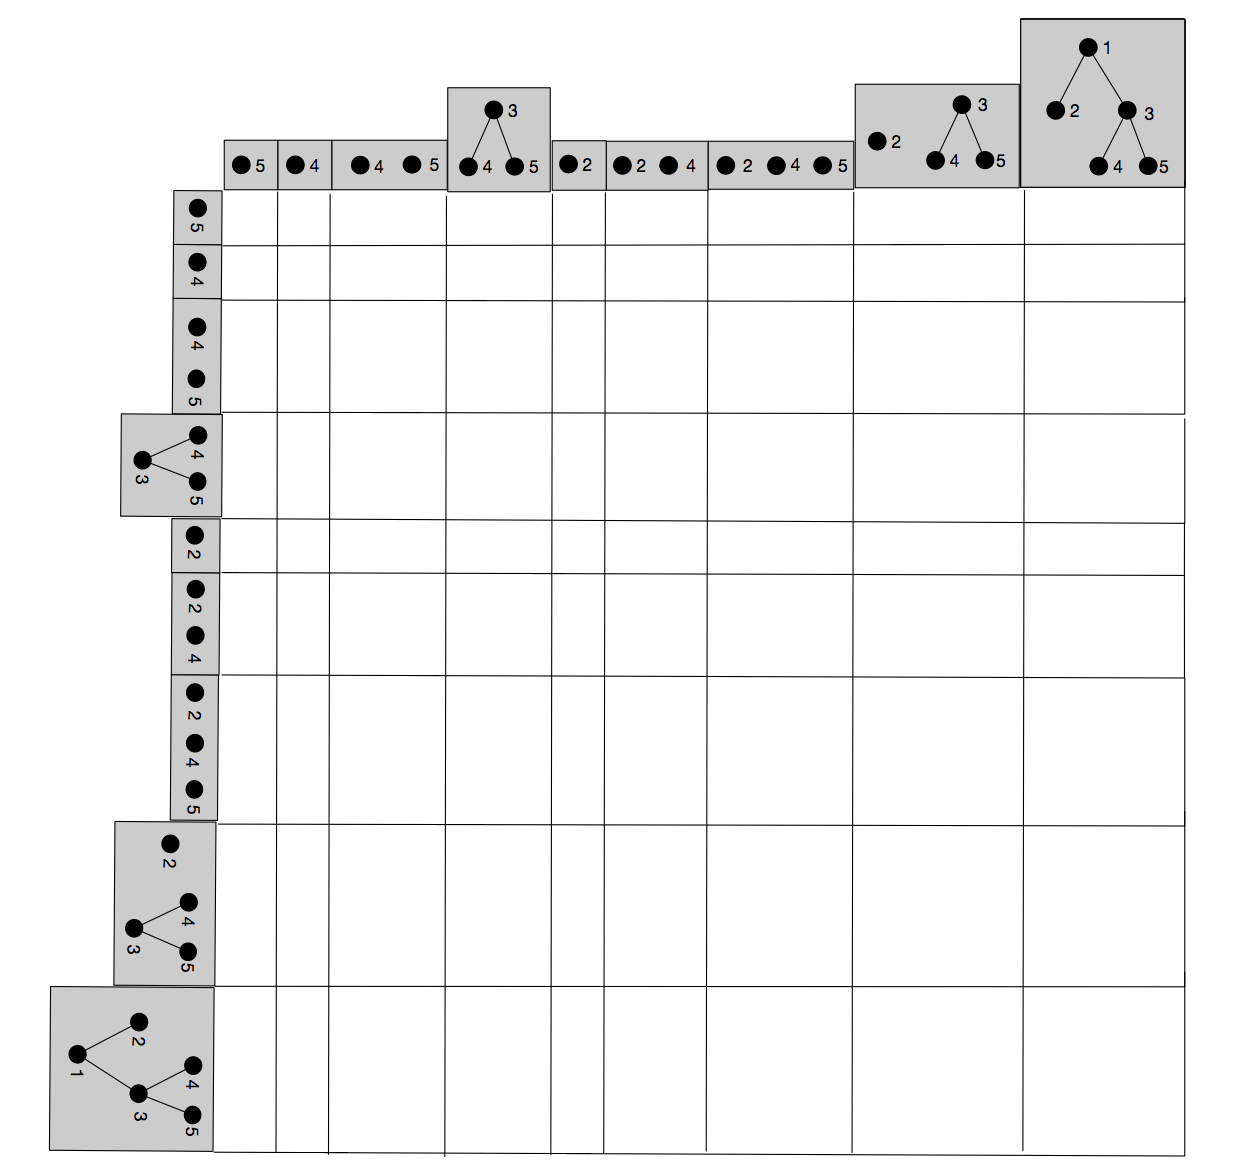
\includegraphics[width=0.5\linewidth]{ForestTable}
	\centering
\end{figure}
\item The upper bound of the post-order enumeration method for the tree edit distance problem is $\mathcal{O}(n^4)$
\end{itemize}
\end{frame}
%------------------------------------------------
\begin{frame}
\frametitle{Improved Algorithmic Path Strategies}
\textbf{Key Ideas:}
\begin{itemize}
\item Different path decomposition creates different number of relevant sub-forests.
\item Take advantage of the overlap among sub-forests that are contained in the same sub-tree, and the overlap of sub-trees as well.
\end{itemize}
\begin{figure}
	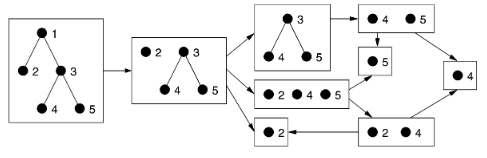
\includegraphics[width=0.6\linewidth]{LeftmostPathDecomposition}
	\centering
\end{figure}
\begin{figure}
	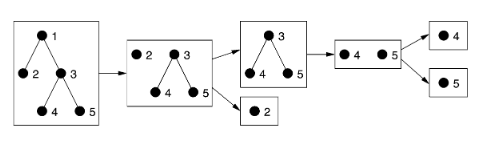
\includegraphics[width=0.6\linewidth]{RightmostPathDecomposition}
	\centering
\end{figure}
\end{frame}
%------------------------------------------------
\begin{frame}
\frametitle{Zhang and Shasha's Algorithm}
\textbf{Key Ideas:}
\begin{itemize}
\item Fixed direction in each recursive calls.
\begin{itemize}
\item Recursive right decomposition - leftmost paths.
\item Recursive left decomposition - rightmost paths.
\end{itemize}
\end{itemize}
\begin{figure}
	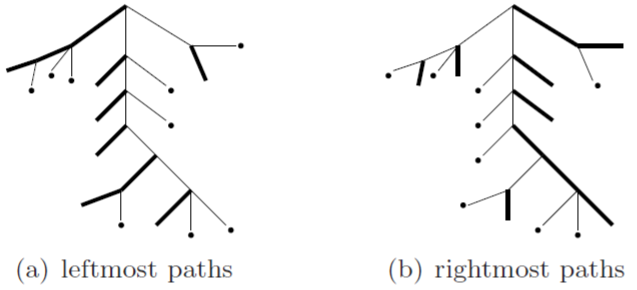
\includegraphics[width=0.7\linewidth]{LeftmostPathandRightmostPath}
	\centering
\end{figure}
\end{frame}
%------------------------------------------------
\subsection{Zhang and Shasha's Algorithm}
\begin{frame}
\frametitle{Zhang and Shasha's Algorithm}
\textbf{Implementation:}
\begin{itemize}
\item Implemented via dynamic programming.
\item Enumerates sub-trees pairs rooted at key roots.
\begin{itemize}
\item Leftmost paths: either tree root or has a left sibling
\item Rightmost paths: either tree root or has a right sibling
\end{itemize}
\item Uses two memorized tables to store intermediate results:
\begin{itemize}
\item a temporary table to store forest-forest distance.% , which is rewrited in each enumerations.
\item a permanent table to store tree-tree distance.
\end{itemize} 
\item Runs in $\mathcal{O}(\left\vert A \right\vert * \left\vert B \right\vert *min\{depth(A), leaves(A)\}*min\{depth(B), leaves(B)\})$ time and $\mathcal{O}(\left\vert A \right\vert * \left\vert B \right\vert)$ space. 
\end{itemize}
\end{frame}
%------------------------------------------------
\subsection{Klein's Algorithm}
\begin{frame}
\frametitle{Klein's Algorithm}
\textbf{Key Ideas:}
\begin{itemize}
\item Zhang and Shasha's algorithm depends on shapes of trees.
\item Heavy node.

\item Heavy paths generate the least number of sub-forests on one tree.
\end{itemize}
\begin{figure}
	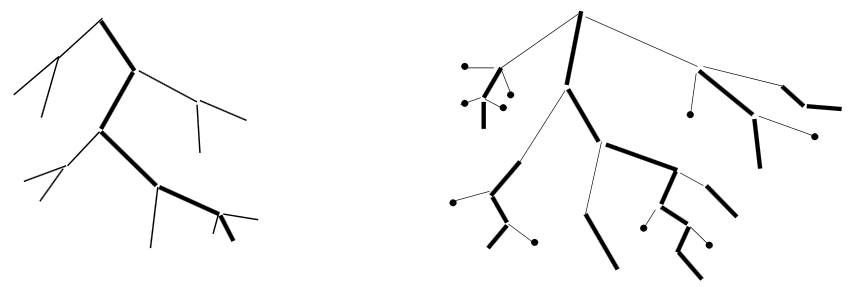
\includegraphics[width=0.8\linewidth]{HeavyPaths}
	\centering
\end{figure}
\end{frame}
%------------------------------------------------
\begin{frame}
\frametitle{Klein's Algorithm}
\textbf{Implementation:}
\begin{itemize}
\item Implemented via dynamic programming.
\item applies heavy paths to the larger tree and fully decomposes the smaller tree.
\item Uses temporary tables to store forest-forest distance and a permanent tables to store tree-tree distance.
\item Runs in $\mathcal{O}(\left\vert A \right\vert \log(\left\vert A \right\vert) * \left\vert B \right\vert^2)$ time using $\mathcal{O}(\left\vert A \right\vert * \left\vert B \right\vert)$ space.
\end{itemize}
\end{frame}
%------------------------------------------------
\subsection{Demaine's Algorithm}
\begin{frame}
\frametitle{Demaine's Algorithm}
\textbf{Key Ideas:}
\begin{itemize}
\item Klein's algorithm consider the shape of one tree with no consideration on the other tree.
\item Heavy paths can be applied on both trees. 
\item Always applies heavy paths on the larger tree. 
\end{itemize}
\textbf{Implementation:}
\begin{itemize}
\item Implemented via dynamic programming.
\item Runs in $\mathcal{O}(\left\vert A \right\vert \left\vert B \right\vert ^ 2(1 + \log(\frac{\left\vert A \right\vert}{\left\vert B \right\vert}))$ time using $\mathcal{O}(\left\vert A \right\vert * \left\vert B \right\vert)$ space.
\end{itemize}
\end{frame}
%------------------------------------------------
\begin{frame}
\frametitle{Conclusion}
\begin{table}
			\centering
			\begin{tabular}{l l l l}
				\toprule
				\textbf{} & \textbf{Time} & \textbf{Space} & \textbf{Comments}\\

				\midrule
				Simple Algorithm &  $\mathcal{O}(n^4)$ & $\mathcal{O}(n^4)$ & first algorithm\\
				Zhang & $\mathcal{O}(n^2\log^2(n))$ & $\mathcal{O}(n^2)$ & efficient for balanced trees \\
				Klein &  $\mathcal{O}(n^3\log(n))$ & $\mathcal{O}(n^2)$ &  no consider smaller trees\\
				Demaine &  $\mathcal{O}(n^3)$ & $\mathcal{O}(n^2)$ & worse case is frequent\\
			\end{tabular}
		\caption{State-of-the-Art Algorithms in the Tree Edit Distance Problem}
\end{table}
\end{frame}
%------------------------------------------------
\section{Algorithmic Improvement}
\begin{frame}
\frametitle{Optimal Root-leaf Path}
\textbf{Key Idea:}
\begin{itemize}
\item heavy paths is a kind of greedy algorithm which usually lead to the local optimum rather than global optimum.
\item quantifies each possible paths and selects the path with the least number of sub-problems is selected
\item implemented via dynamic programming.
\item Preprocessing time  is bounded by $\mathcal{O}(\left\vert A \right\vert \left\vert B \right\vert)$
% hard-coded stratgies are bad for specific tree shapes
\end{itemize}
\end{frame}
%------------------------------------------------
\begin{frame}
\frametitle{Relevant Leftmost/Rightmost/Special Sub-forests}
\begin{itemize}
\item Path decomposition $\to$ relevant sub-forests %are forests created in each recursive call.
\item Recursive leftmost path decomposition $\to$ relevant leftmost sub-forests %are forests obtaining from applying the leftmost path decomposition to the whole tree and its relevant sub-trees.
\begin{figure}
	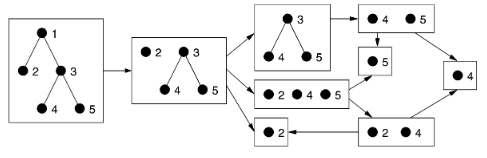
\includegraphics[width=0.5\linewidth]{LeftmostPathDecomposition}
	\centering
\end{figure}
\item Recursive rightmost path decomposition $\to$ relevant rightmost sub-forests %are forests obtaining from applying the rightmost path decomposition to the whole tree and its relevant sub-trees.
\begin{figure}
	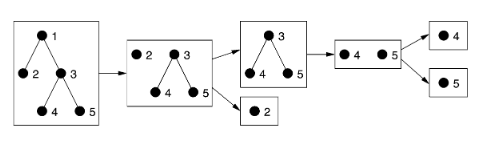
\includegraphics[width=0.5\linewidth]{RightmostPathDecomposition}
	\centering
\end{figure}
\item Full decomposition $\to$ relevant special sub-forests %are forests obtaining from the full decomposition.
\end{itemize}
\end{frame}
%------------------------------------------------
\begin{frame}
\frametitle{Relevant Leftmost/Rightmost/Special Sub-forests}
Let T be a tree of the form $l(T_1 \comp \cdots \comp T_n)$ and the size of T is $n$, 
\begin{itemize}
\item The Number of Relevant Leftmost Sub-forests($\#left(T)$)
\begin{equation*}
\#left(T) = \left\vert T \right\vert - \left\vert T_1 \right\vert + \sum_{i=1}^{n}\#left(T_i)
\end{equation*}
\item The Number of Relevant Rightmost Sub-forests($\#right(T)$)
\begin{equation*}
\#right(T) = \left\vert T \right\vert - \left\vert T_n \right\vert + \sum_{i=1}^{n}\#right(T_i)
\end{equation*}
\item Relevant Special Sub-forests($\#special(T)$)
\begin{equation*}
\#spec(T) = \frac{n(n+3)}{2} - \sum_{i \in T}\left\vert T(i) \right\vert
\end{equation*}
\end{itemize}
\end{frame}
%------------------------------------------------
\begin{frame}
\frametitle{Status of a Node in a Tree}
Let T be a tree with a root-leaf path, 
\begin{itemize}
\item Free node: the node is the root of T, or is not on the root-leaf path.
\item Left node:the node is on the root-leaf path and is the leftmost child of its parent.
\item Right node:the node is on the root-leaf path and is the rightmost child of its parent.
\item All node:the node is on the root-leaf path and is neither the leftmost child nor the rightmost child of its parent.
\end{itemize}
\begin{figure}
	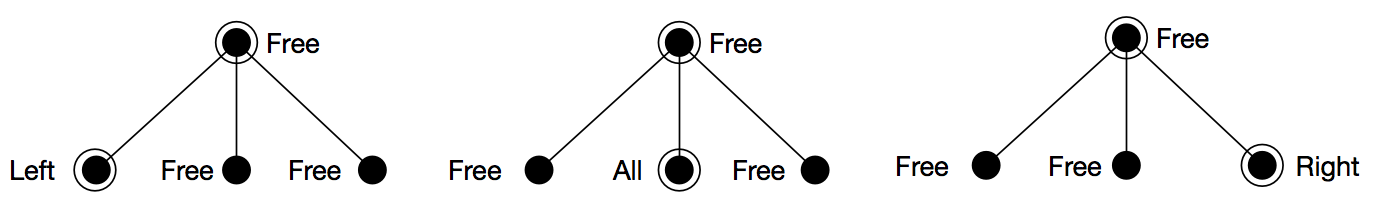
\includegraphics[width=1.0\linewidth]{Nodes}
	\centering
\end{figure}
\end{frame}
%------------------------------------------------
\begin{frame}
\frametitle{Quantify the Number of Sub-Problem}
\begin{itemize}
\item Seven memorized tables to store intermediate results.
\begin{itemize}
\item Free
\item LeftA
\item RightA
\item AllA
\item LeftB
\item RightB
\item AllB
\end{itemize}
\item Dynamic programming.
\end{itemize}
\end{frame}
%------------------------------------------------
\begin{frame}
\frametitle{Quantify the Number of Sub-Problem}
Let A be a tree with a root-leaf path and B be another tree,
\begin{columns}[c]
\column{.5\textwidth}
\begin{figure}
	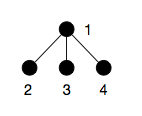
\includegraphics[width=0.3\linewidth]{treeA}
	\centering
\end{figure}
\column{.5\textwidth}
\begin{figure}
	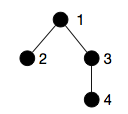
\includegraphics[width=0.3\linewidth]{treeB}
	\centering
\end{figure}
\end{columns}
\end{frame}
%------------------------------------------------
\begin{frame}
\frametitle{Quantify the Number of Sub-Problem}
Let A be a tree with a root-leaf path and B be another tree.
\begin{figure}
	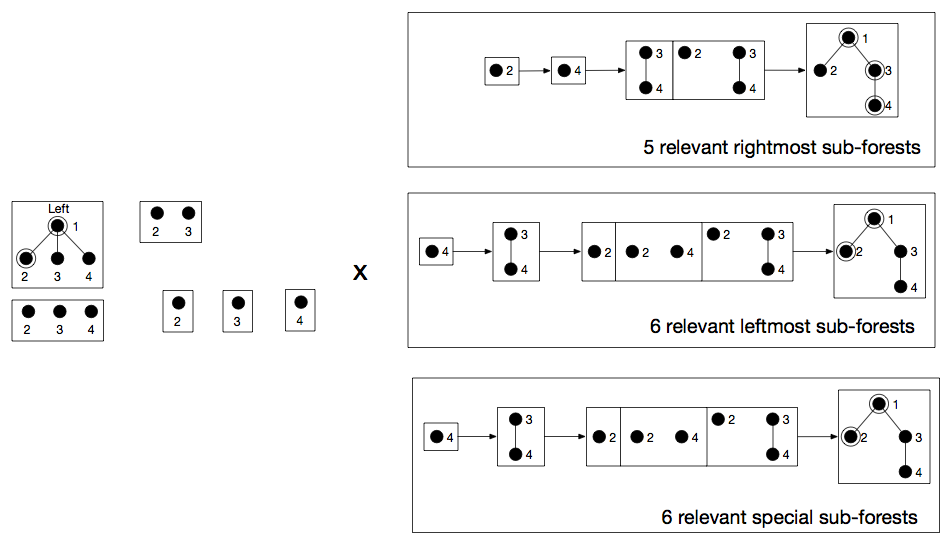
\includegraphics[width=0.7\linewidth]{leftleft}
	\centering
\end{figure}
\begin{eqnarray*}
\#leftA(1, 1) &=& Free(3, 1) + Free(4, 1) + LeftA(2, 1)\\
&+& \left\vert A - A(2) \right\vert * \#left(B) \\
&=& \#left(B) + \#left(B) + \#left(B) + 3 * \#left(B)
\end{eqnarray*}
\end{frame}
%------------------------------------------------
\begin{frame}
\frametitle{Quantify the Number of Sub-Problem}
Let A be a tree with a root-leaf path and B be another tree.
\begin{figure}
	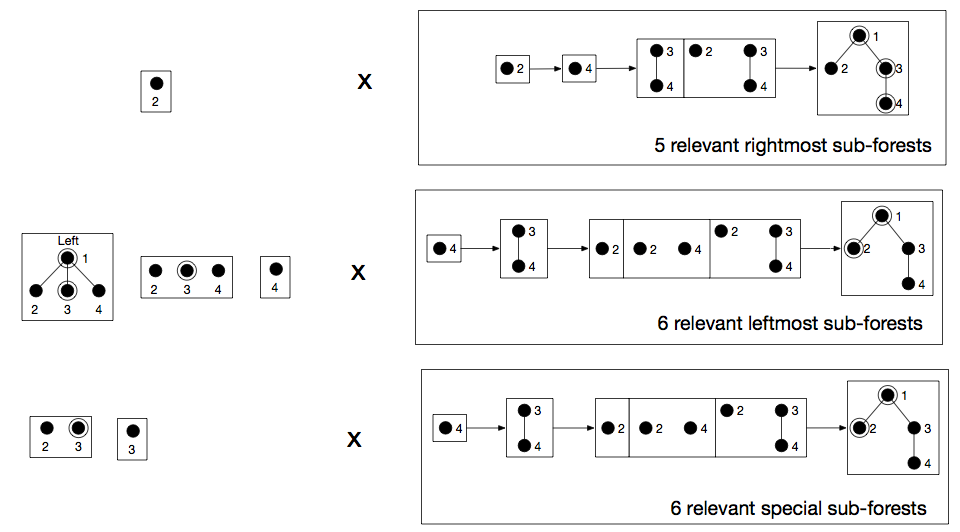
\includegraphics[width=0.7\linewidth]{leftmid}
	\centering
\end{figure}
\begin{eqnarray*}
\#leftA(1, 1) &=& Free(2, 1) + Free(4, 1) + AllA(3, 1)\\
&+& \left\vert 1 + A(4) \right\vert * \#left(B) + \left\vert A(2) \right\vert * \#special(B) \\
&=& \#right(B) + \#left(B) + \#special(B)\\
&+&  \#special(B) + 2 * \#left(B)
\end{eqnarray*}
\end{frame}
%------------------------------------------------
\begin{frame}
\frametitle{Quantify the Number of Sub-Problem}
Let A be a tree with a root-leaf path and B be another tree.
\begin{figure}
	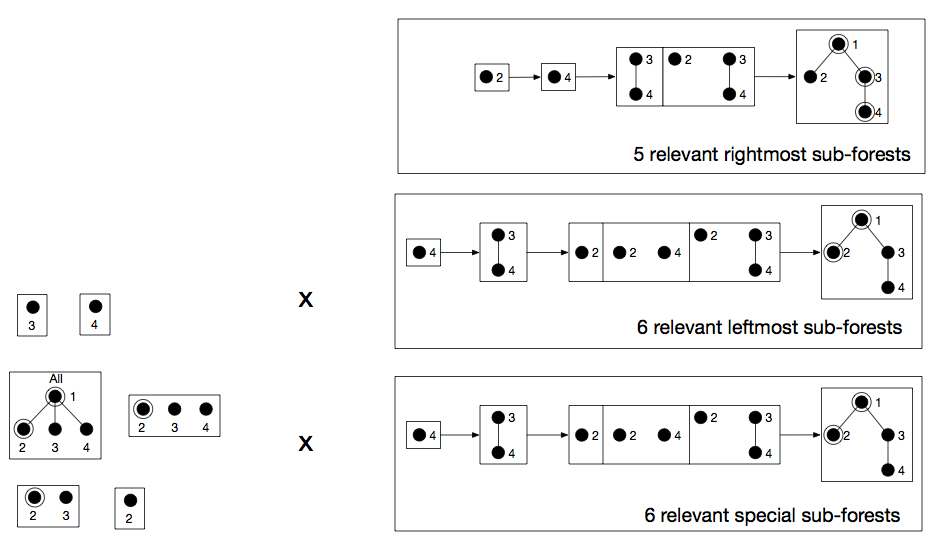
\includegraphics[width=0.7\linewidth]{allleft}
	\centering
\end{figure}
\begin{eqnarray*}
\#AllA(1, 1) &=& Free(3, 1) + Free(4, 1) + AllA(2, 1)\\
&+& \left\vert A - A(2) \right\vert * \#special(B)\\
&=& \#left(B) + \#left(B) + \#special(B) + 3 * \#special(B)\\
\end{eqnarray*}
\end{frame}
%------------------------------------------------
\begin{frame}
\frametitle{Vertical Reduction on Trees}
\textbf{Key Ideas:}

\begin{itemize}
\item A large number of non-branching nodes can be compressed into one node.
\begin{figure}
	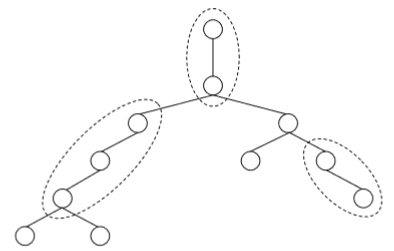
\includegraphics[width=0.25\linewidth]{VComponent}
	\centering
\end{figure}
\item The compact representation of the original tree can aid in improving the running time for computing the tree edit distance.
\begin{figure}
	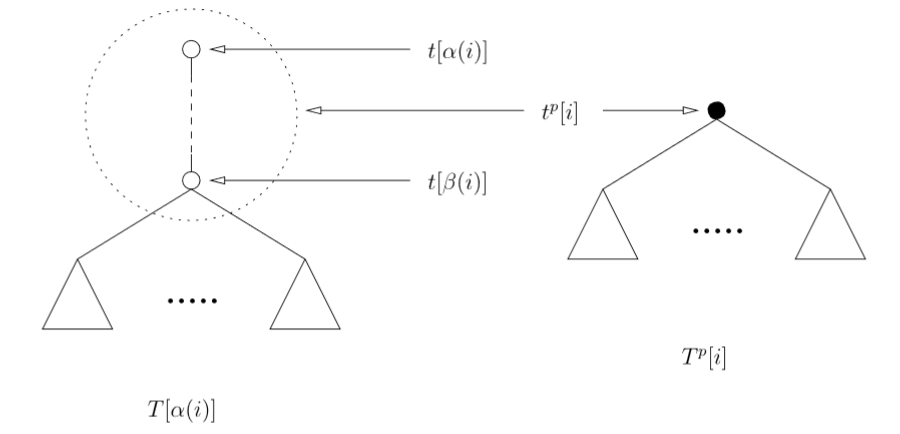
\includegraphics[width=0.45\linewidth]{VReduction}
	\centering
\end{figure}
\item $T \to \widetilde{T}$
\end{itemize}
\end{frame}
%------------------------------------------------
\begin{frame}
\frametitle{Algorithm}
\textbf{Forest-to-Forest Distance}:
\begin{figure}
	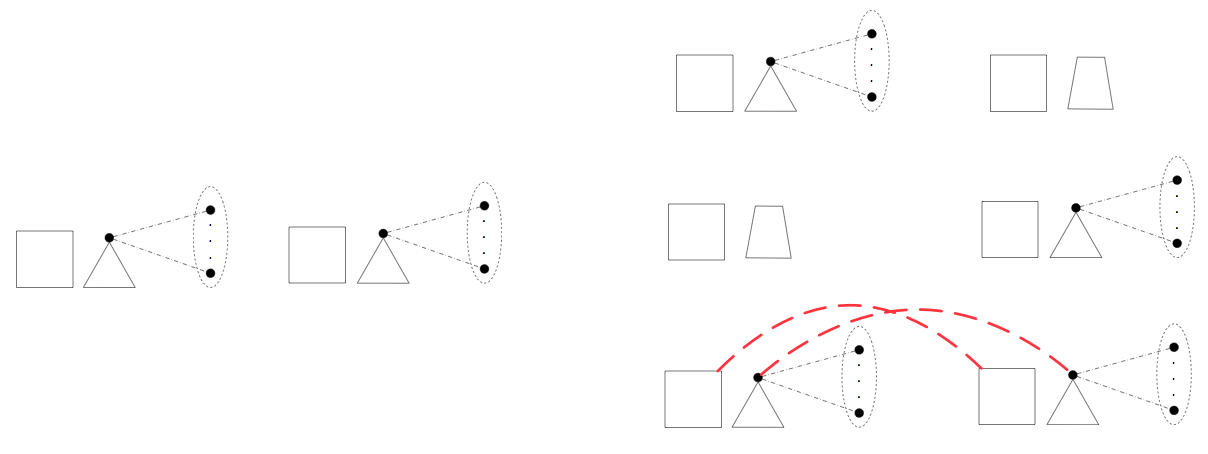
\includegraphics[width=1.0\linewidth]{forestforestcompressed}
	\centering
\end{figure}

\end{frame}
%------------------------------------------------
\begin{frame}
\frametitle{Algorithm}
\textbf{Tree-to-Tree Distance}:
\begin{itemize}
\item Compute $d(\widetilde{T_1}, \widetilde{T_2}^{\comp})$
\begin{figure}
	\includegraphics[width=0.85\linewidth]{TreeInitial}
	\centering
\end{figure}
\item The computation of $d(\widetilde{T_1}^{\comp}, \widetilde{T_2})$ is symmetric.
\end{itemize}
\end{frame}
%------------------------------------------------
\begin{frame}
\frametitle{Algorithm}
\textbf{Tree-to-Tree Distance}:
\begin{itemize}
\item Compute $d(\widetilde{T_1}, \widetilde{T_2})$
\begin{figure}
	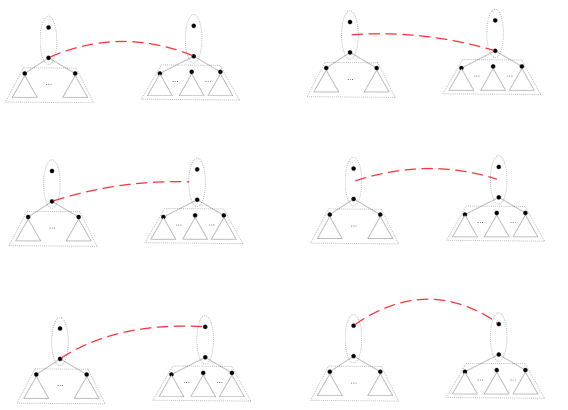
\includegraphics[width=0.85\linewidth]{treetreecompressed}
	\centering
\end{figure}
\end{itemize}
\end{frame}
%------------------------------------------------
\begin{frame}
\frametitle{Implementation}
\begin{itemize}
\item three memorized tables to store intermediate results:
\begin{itemize}
\item $D_t$: a $(\left\vert T_1 \right\vert + 1) * (\left\vert T_2 \right\vert + 1)$ two dimensional permanent array.
\item $\widetilde{D}_t$: a $(\left\vert \widetilde{T}_1 \right\vert + 1) * (\left\vert \widetilde{T}_2 \right\vert + 1)$ two dimensional permanent array.
\item $\widetilde{D}_f$: a $(\left\vert \widetilde{T}_1 \right\vert + 1) * (\left\vert \widetilde{T}_2 \right\vert  + 1)$ two dimensional temporary array.
\end{itemize}
\item Dynamic programming.
\end{itemize}
\end{frame}
%------------------------------------------------
\begin{frame}
\frametitle{RNA}
\begin{itemize}
\item RNA is an essential molecule in organisms.
\begin{itemize}
\item Cellular organisms
\item Viruses
\end{itemize}
%Cellular organisms use messenger RNA (mRNA) to convey genetic information.
%Viruses encode their genetic information using an RNA genome.
\item RNA is assembled as a chain of nucleotides. 
\begin{figure}
	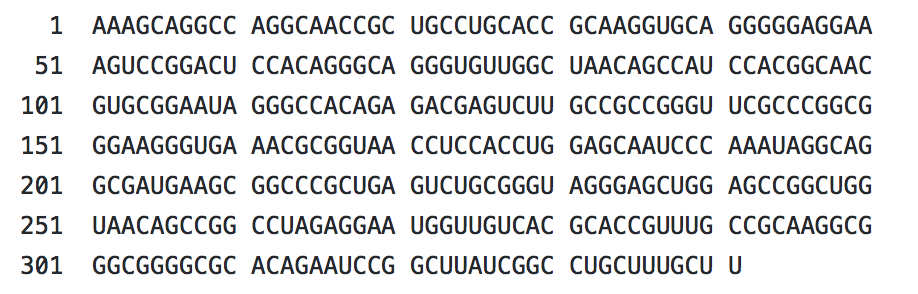
\includegraphics[width=0.8\linewidth]{RNASequence}
	\centering
\end{figure}
%can be represented as finite-length string over an alphabet. The alphabet is a set containing four symbols A U G C, which represents four kinds of nucleotides. 
\item RNA is unstable. 
%Unlike the double-strand struture of DNA, RNA is a single-strand and thus it is easaily fold back onto itself by means of hydrogen bonding, resulting in the secondary structure. 
\begin{columns}[c]
\column{.5\textwidth}
\begin{figure}
	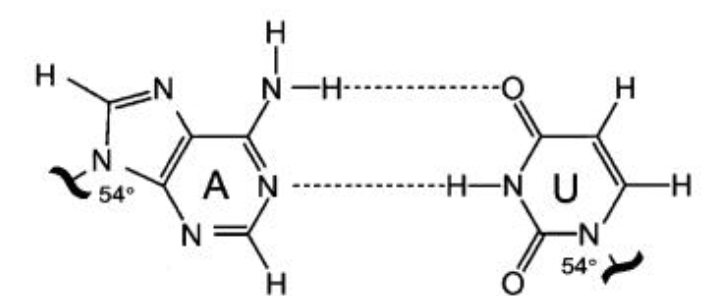
\includegraphics[width=0.8\linewidth]{AUBasePair}
	\centering
\end{figure}
\column{.5\textwidth}
\begin{figure}
	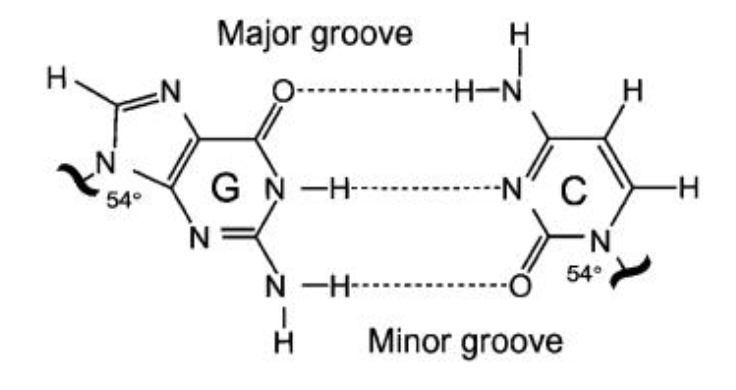
\includegraphics[width=0.8\linewidth]{GCBasePair}
	\centering
\end{figure}
\end{columns}
\end{itemize}
\end{frame}
%------------------------------------------------
\section{Applications in the RNA Secondary Structure Comparison}
\begin{frame}
\frametitle{RNA Secondary Structure}
\begin{itemize}
\item a list of base pairs satisfies the following constraints:
\begin{itemize}
\item A base cannot participate in more than one base pair,
\item No two base pairs cross.
\end{itemize}
\begin{figure}
	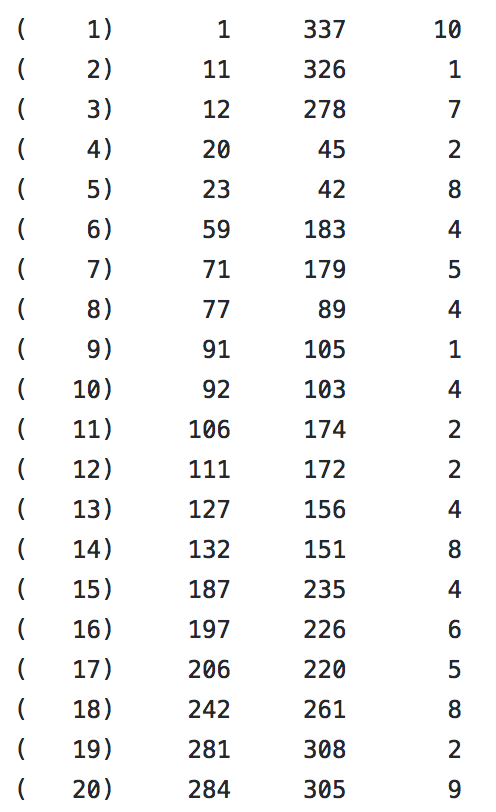
\includegraphics[width=0.35\linewidth]{BasePairs}
	\centering
\end{figure}
\end{itemize}
\end{frame}
%------------------------------------------------
\begin{frame}
\frametitle{RNA Secondary Structure Representation}
\begin{itemize}
\item String representation
\begin{figure}
	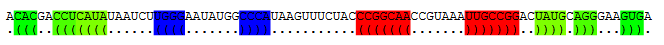
\includegraphics[width=1.0\linewidth]{RNAST1}
	\centering
\end{figure}
\item Graph representation
\begin{figure}
	\includegraphics[width=0.8\linewidth]{RNAST2}
	\centering
\end{figure}
%fold into a circle continue fold it into a 2D structure
%stem and loop
\end{itemize}
\end{frame}
%------------------------------------------------
\begin{frame}
\frametitle{Tree Representation of the RNA Secondary Structure}
\begin{itemize}
\item Base pair labelling
\begin{table}
			\centering
			\begin{tabular}{l l}
				\toprule
				\textbf{Base Pairs} & \textbf{Label}\\
				\midrule
				$A = U$ & F\\
				$G \equiv C$ & J\\
				$U = A$ & P\\
				$C \equiv G$ & M\\
			\end{tabular}
		\caption{The Label of Base Pair}
\end{table}
\item Tree representation
\end{itemize}
\end{frame}
%------------------------------------------------
\begin{frame}
\frametitle{Tree Representation of the RNA Secondary Structure}
\begin{figure}
	\includegraphics[width=0.6\linewidth]{RNAST3}
	\centering
\end{figure}
\end{frame}
%------------------------------------------------
\begin{frame}
\frametitle{Experiment}
\begin{figure}
	\includegraphics[width=1.0\linewidth]{AlcaligenesString}
	\centering
\end{figure}
\begin{figure}
	\includegraphics[width=1.0\linewidth]{StreptomycesString}
	\centering
\end{figure}
\end{frame}
%------------------------------------------------
\begin{frame}
\frametitle{Experiment}
\begin{figure}
	\includegraphics[width=0.8\linewidth]{RNAGraphExample}
	\centering
\end{figure}
\end{frame}
%------------------------------------------------
\begin{frame}
\frametitle{Experiment Result}
\begin{figure}
	\includegraphics[width=1.0\linewidth]{AlignmentResult}
	\centering
\end{figure}
\end{frame}
\section{Evaluation}
\begin{frame}
\frametitle{Evaluation}
Tree size: 246 and 282
\begin{table}
			\centering
			\begin{tabular}{l l l}
				\toprule
				\textbf{Algorithm} & \textbf{$\#Rel.sub$} &\textbf{Time[sec]}\\
				\midrule
				$Zhang-L$ & 849282 & 0.08\\
				$Zhang-R$ & 2039089 & 0.13\\
				$Demaine$ & 7175224 & 0.65\\
				$Our\ Algorithm(Before\ Compression)$ & 553526 & 0.04\\
				$Zhang-L(Compressed)$ & 428766 & 0.05\\
				$Zhang-R(Compressed)$ & 686562 & 0.05\\
				$Our\ Algorithm(After\ Compression)$ & 291329 & 0.03\\
			\end{tabular}
\end{table}
\end{frame}
\begin{frame}
\frametitle{Evaluation}
Tree size: 1041 and 1012
\begin{table}
			\centering
			\begin{tabular}{l l l}
				\toprule
				\textbf{Algorithm} & \textbf{$\#Rel.sub$} &\textbf{Time[sec]}\\
				\midrule
				$Zhang-L$ & 41889364 & 3.2\\
				$Zhang-R$ & 42972591 & 3.3\\
				$Demaine$ & 273276733 & 20.98\\
				$Our\ Algorithm(Before\ Compression)$ & 32254346 & 2.3\\
				$Zhang-L(Compressed)$ & 17769036 & 0.47\\
				$Zhang-R(Compressed)$ & 18154025 & 0.51\\
				$Our\ Algorithm(After\ Compression)$ & 13546825 & 0.34\\
			\end{tabular}
\end{table}
\end{frame}
%------------------------------------------------
\section{Conclusion}
\begin{frame}
\frametitle{Conclusion}
\begin{itemize}
\item Tree edit distance quantifies the similarity between two ordered labelled trees. 
\item Three kinds of root-leaf path are introduced to take the advantages of the overlapping relevant sub-forests and sub-trees in different ways.
\item The optimal root-leaf path can be found via dynamic programming and can be used for the tree edit distance problem.
\item The vertical reduction on trees can significantly reduced the running time.
\item The comparison between RNA secondary structures is an application of the tree edit distance.
\item Our strategies on compressed trees are by far the best decomposition strategy, creating the least number of relevant sub-problems.
\end{itemize}
\end{frame}
\begin{frame}
Thank you. Questions?
\end{frame}

%------------------------------------------------
% Back up slides
%------------------------------------------------
\begin{frame}
\frametitle{Path Decomposition}
\begin{itemize}
\item Leftmost path decomposition
\begin{figure}
	\includegraphics[width=0.6\linewidth]{LeftmostPathDecomposition}
	\centering
\end{figure}
\item Rightmost path decomposition
\begin{figure}
	\includegraphics[width=0.6\linewidth]{RightmostPathDecomposition}
	\centering
\end{figure}
\end{itemize}
\end{frame}
%------------------------------------------------
\begin{frame}
\frametitle{Bottom-up Enumeration}
Two orders of the enumeration of the path decomposition:
\begin{itemize}
\item LR-postorder enumeration%enumate the rightmost root in LR-postorder and fix it, then enumerate the leftmost root in RL-postorder.
\begin{figure}
	\includegraphics[width=0.9\linewidth]{LRPostorder}
	\centering
\end{figure}
\item RL-postorder enumeration%fenumerate the leftmost root in RL-postorder and fix it, then enumerate the rightmost root in LR-postorder.
\begin{figure}
	\includegraphics[width=1.0\linewidth]{RLPostorder}
	\centering
\end{figure}
\end{itemize}
\end{frame}
%------------------------------------------------
\begin{frame}
\frametitle{Matching in Trees}
\begin{itemize}
\item \textbf{Input:}
Two labelled ordered trees $T$ and $P$.
\item \textbf{Constraints: }
\begin{itemize}
\item One-to-one relationship
\item Sibling order is preserved.
\begin{figure}
	\includegraphics[width=1.0\linewidth]{SiblingOrderPreserved}
	\label{Sibling Order is Preserved} 
	\centering
\end{figure}
\item Ancestor order is preserved.
\begin{figure}
	\includegraphics[width=1.0\linewidth]{AncestorOrderPreserved}
	\label{Ancestor Order is Preserved} 
	\centering
\end{figure}
\end{itemize}
\item \textbf{Output:}
Mapping between $T$ and $P$. 
\end{itemize}
\end{frame}	
%------------------------------------------------
\end{document}